\documentclass[10pt]{beamer}

\setbeamertemplate{note page}[default]
%\setbeameroption{hide notes}
\setbeameroption{show notes}


\usetheme[progressbar=frametitle]{metropolis}
\usepackage{appendixnumberbeamer}

\usepackage{booktabs}
\usepackage[scale=2]{ccicons}

\usepackage{pgfplots}
\usepgfplotslibrary{dateplot}
\usepackage{multicol}
\setlength{\columnsep}{1.5cm}

\usepackage{animate}
\usepackage{lmodern}
\usepackage[T1]{fontenc}
\usepackage{mathtools}
\usepackage{graphicx}
\usepackage{caption}

\definecolor{set1}{RGB}{228, 26, 28}
\definecolor{set2}{RGB}{77, 175, 74}
\definecolor{set3}{RGB}{255, 127, 0}
\definecolor{set4}{RGB}{166, 86, 40}
\definecolor{set5}{RGB}{153, 153, 153}

\usepackage{xspace}
\newcommand{\themename}{\textbf{\textsc{metropolis}}\xspace}

\newcommand\Fontvi{\fontsize{8}{9}\selectfont}
\newcommand\Fontvr{\fontsize{6}{7}\selectfont}

\setbeamerfont{parent A}{size=\small}


\title{Study Design}
\subtitle{Digital Transformation of Healthcare}
% \date{\today}
\date{}
\author{Michoel Snow, MD PhD}
\institute{Center for Health Data Innovations}
% \titlegraphic{\hfill\includegraphics[height=1.5cm]{logo.pdf}}

\begin{document}

\maketitle


\begin{frame}{Who are we?}
	\begin{columns}
		\begin{column}{0.5\textwidth}
			\begin{itemize}
				\item Center for Health Data Innovations (CHDI) 
				\begin{itemize}
					\item formerly, the Clinical Research Informatics (CRI) core
				\end{itemize}
				\item Part of both Einstein and Montefiore 
				\item Develop infrastructure based on informatics technologies
				\item Links Einstein's translation science engine to Montefiore's learning healthcare system
			\end{itemize}	
		\end{column}
		\begin{column}{0.5\textwidth}
			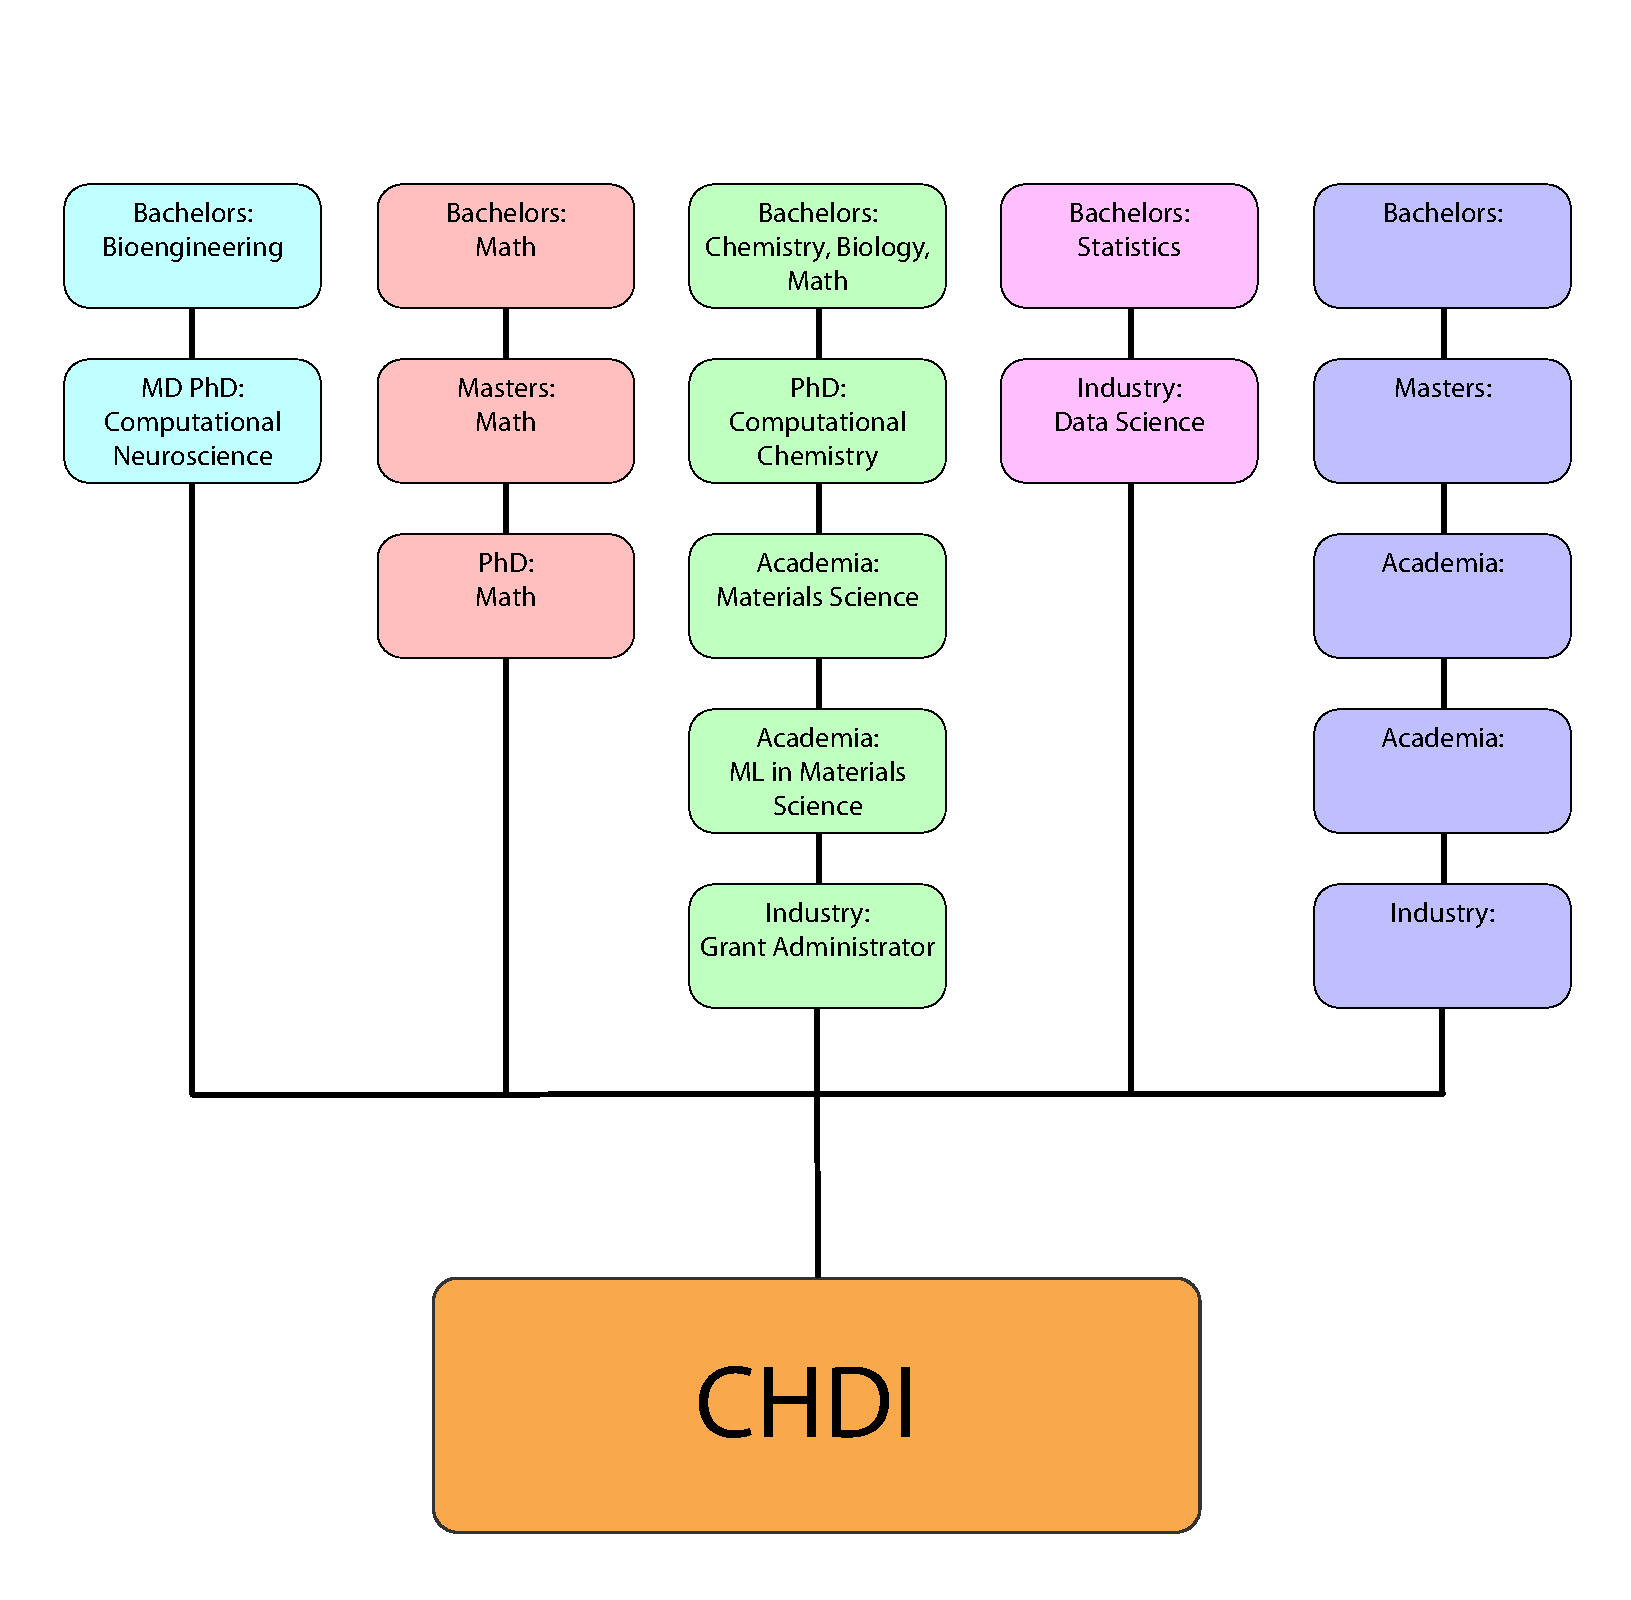
\includegraphics[width=1\columnwidth]{images/data_science_progression.pdf}	
		\end{column}
	\end{columns}
\end{frame}

\begin{frame}{What do we do?}
	\begin{itemize}
		\item PROOFcheck
			\begin{itemize}
					\item Department - Critical Care
					\item Respiratory failure prediction
					\item EMR based alerts
			\end{itemize}
		\item Metastatic Epidural Spinal Cord Compression
			\begin{itemize}
				\item Department - Radiation Oncology
				\item Early identification and remediation of spinal met progression
			\end{itemize}
		\item Outpatient Appointment Attendance 
			\begin{itemize}
				\item Department - Medicine
				\item Determine the probability of a patient not showing up to their appointment
				\item Optimize patient appointments
			\end{itemize}
	\end{itemize}
	
\end{frame}

\begin{frame}{Digital Transformation of Healthcare}
	\small
	\begin{itemize}
		\item What kind of questions can I answer using automatically collected data?
		\item What kind of data is collected by the hospital and how can I access the data?
		\item How much will it cost/save the hospital to implement the study as well as act on its results?
		\item What do I need to consider when designing a study using patient data? 
		\item How can I integrate automatic systems with collaborators to collect the desired data?
		\item How do I transform the data from its collected format to a format useful for analysis?
		\item How can I integrate the results of my study within the hospital system?
	\end{itemize}
\end{frame}


\begin{frame}{Bioinformatics Pipeline}
	\begin{center}
		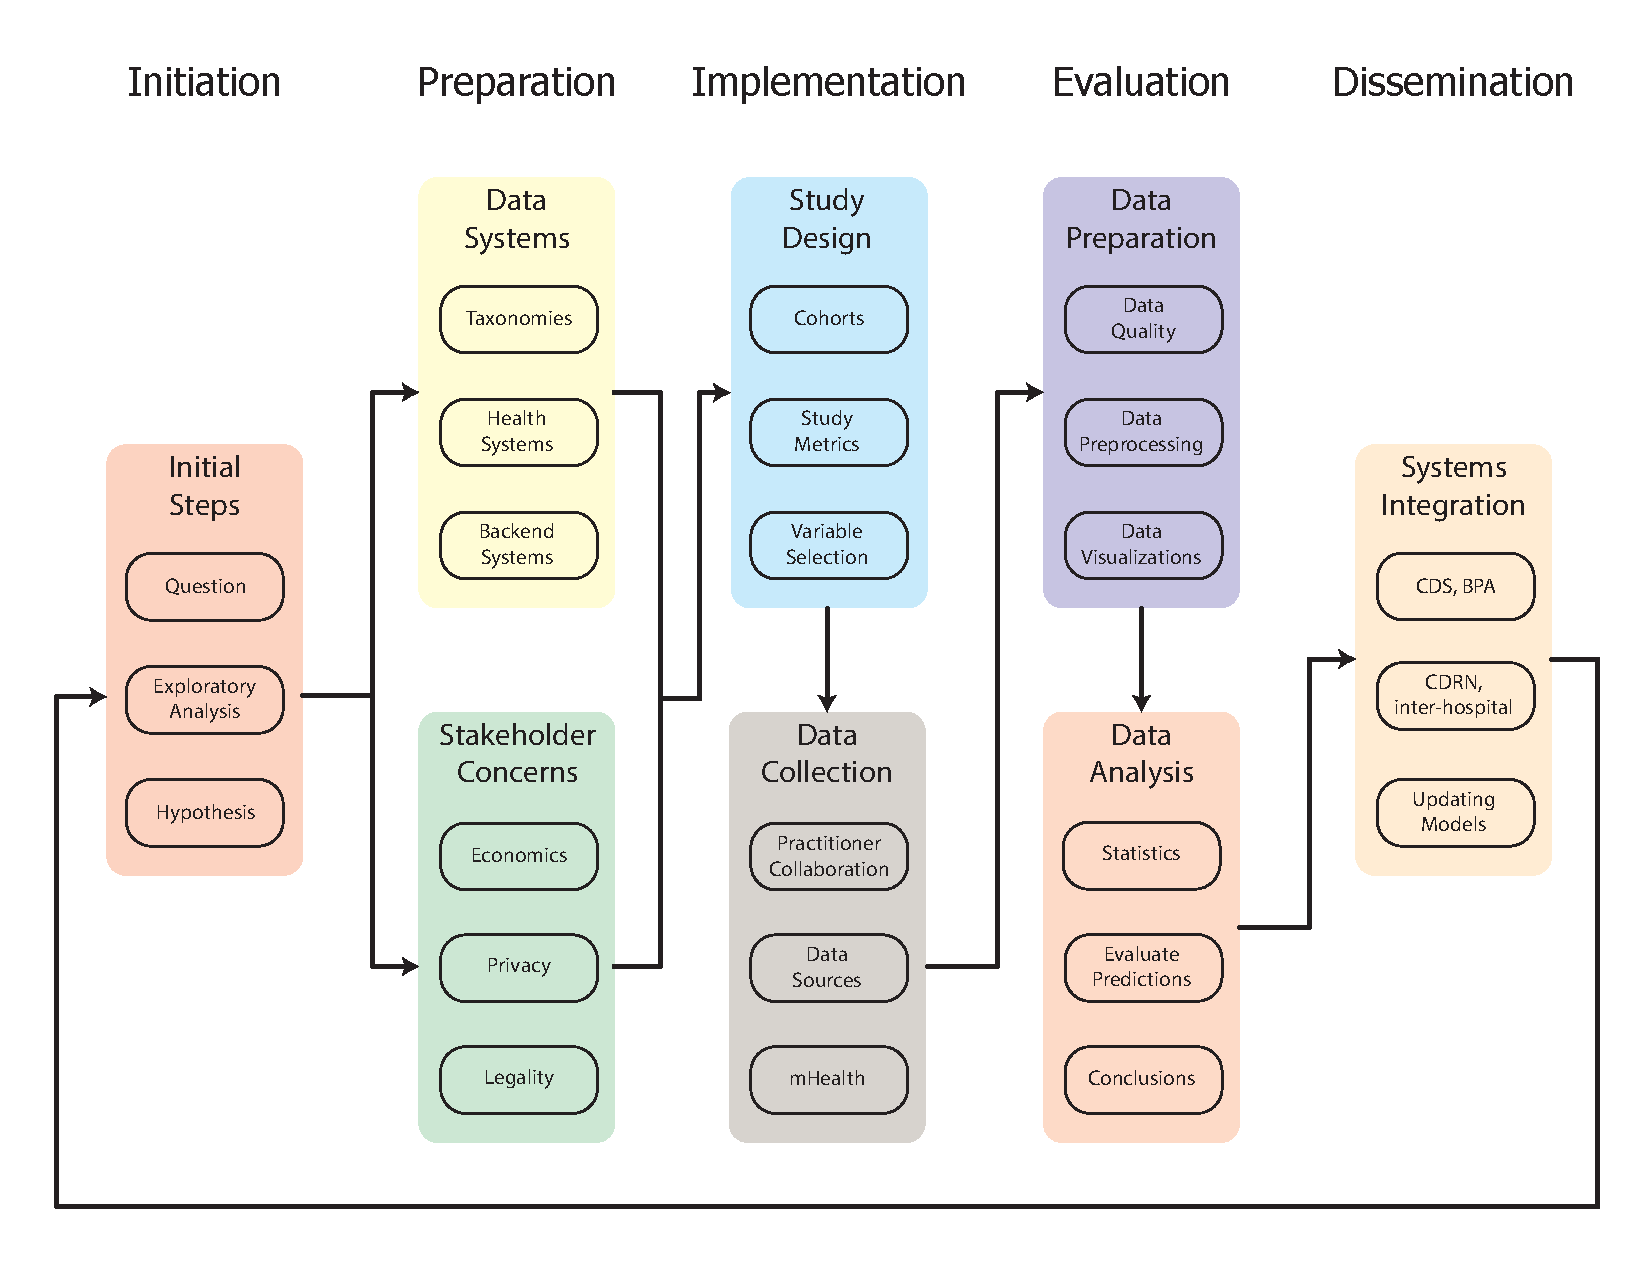
\includegraphics[width=0.8\textwidth]{images/informatics_pipeline.pdf}	
	\end{center}
	\begin{itemize}
		\item Who has been involved in any of these steps?
	\end{itemize}
\end{frame}


\begin{frame}{Study Design}
	\begin{center}
		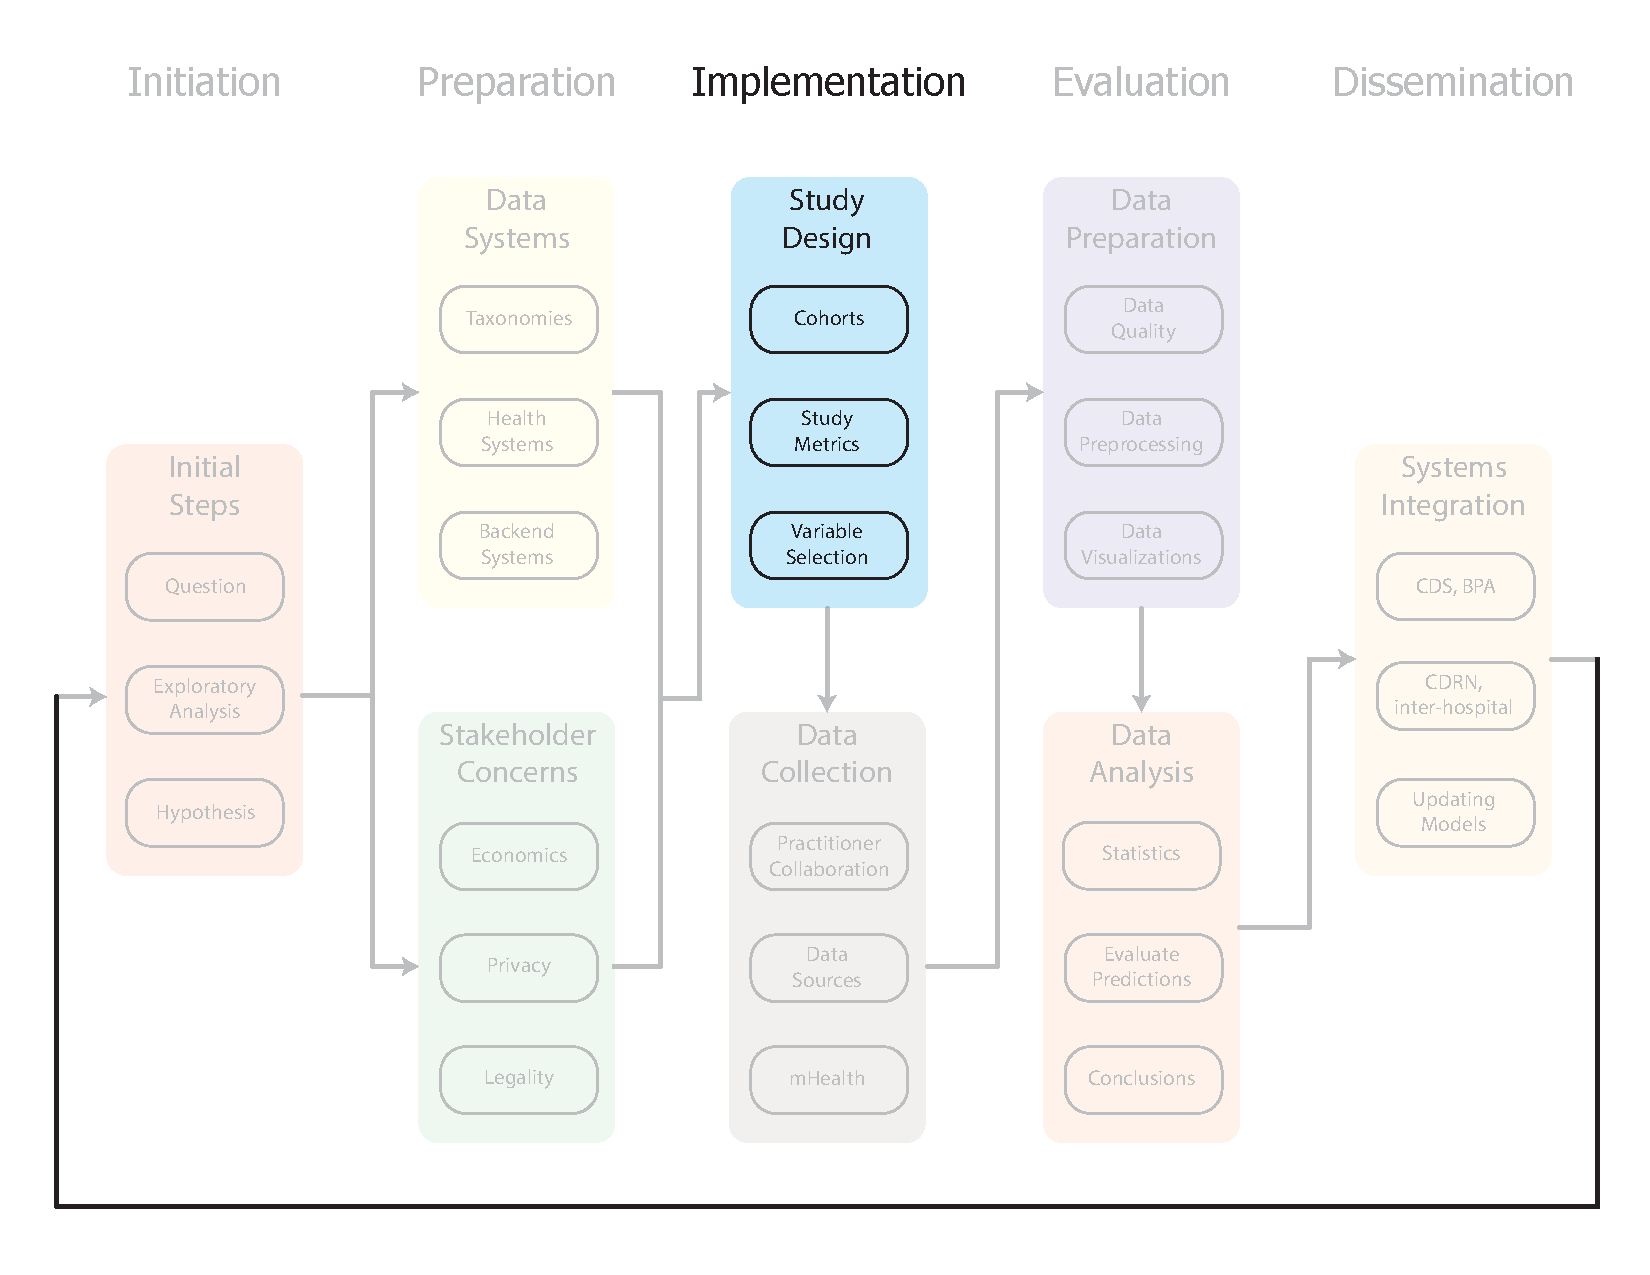
\includegraphics[width=0.8\textwidth]{images/informatics_pipeline_studydesign.pdf}
	\end{center}
\end{frame}


\begin{frame}{Medication Reconciliation}
	\begin{itemize}
		\item Medication reconciliation (Med Rec) is the process of
		\begin{itemize}
			\item Comparing a patient's medication orders to all of the medications they have been taking
			\item Understanding why they're taking each medication
			\item Comparing that list against new orders
		\end{itemize} 
		\item The goal of Med Rec is to provide correct medications to the patient at all transition points within the hospital.		   
	\end{itemize}
\end{frame}

\begin{frame}{Medication Reconciliation}
	\begin{itemize}
		\item According to The Institute of Safe Medication Practice, Med Rec has the potential to eliminate
		\begin{itemize}
			\item 50\% of medication errors
			\item 20\% of adverse medical events
		\end{itemize}
		\item Care providers in Montefiore write 
		\begin{itemize}
			\item About 4 million prescriptions a year (averages out to more than 10,000 a day)
			\item Prescriptions to over 400,000 different patients
			\item Prescriptions for more than 11,000 different medications
		\end{itemize}		   
	\end{itemize}
\end{frame}

\begin{frame}{Med Rec Case Study - Definitions}
	Roses hospital wants to develop a pilot Med Rec system in their Pediatrics department.  You are working with a team of institutional stakeholders tasked with comparing the pre- and post-implementation effects of this system.  You meet with the bioinformatics core to discuss the data collection for the study. As the domain knowledge expert, they ask you following questions: 
	\begin{itemize}
		\item \textcolor<2->{gray}{What qualifies as an adverse drug event (ADE)?}
		\item \textcolor<2->{gray}{What qualifies as a medication error?}
		\item \textcolor<2->{gray}{How would you sub-classify each and where do they overlap?}
		\item<2-> \textcolor<3->{gray}{At what points along the pathway from prescription to ingestion can medication errors occur?}
		\item<2-> \textcolor<3->{gray}{How do you identify and retrace a medication error? An ADE?}
		\item<3-> What is the goal of Med Rec with respect to medication errors? ADEs?
	\end{itemize}	
	\note[item]<1>{\footnotesize{an ADE is an injury due to a medication, e.g., cough due to ACE-I in pt w/o hx of cough, nausea after tamiflu, anaphylaxis due to allergy}}
	\note[item]<1>{A medication error is any mistake along the path of ordering, transcribing, dispensing, administrating, and monitoring, e.g., docusate given 2 hours late (harmless), critical abx never given (harmful), wrong medication given(anywhere from harmless to fatal), ...} 	
	\note[item]<1>{Medication errors range from minor, which have little or no harm potential (late docusate) and are not ADEs, to possible, which could have caused injury but did not, either because they were caught in time or the pt did not have a negative rxn (even if they should have) and these are termed potential ADEs, to fatal which are ADEs}
	\note[item]<1>{ADEs are split into potential ADEs, which are always medication errors but were either intercepted or non-injurious, preventable ADEs which are the result of medication errors and non-preventable ADEs, which are not the result of medication errors, such as allergic rxn in a heretofore non-allergic pt}
	\note[item]<2>{Prescription writing (autocomplete, autofill, patient charts, dosing, allergies), filling prescription (wrong medication, medication interactions, allergies), prescription handoff, administration (route, dosing, delay), patient ingestion (misinterpret instructions, ignore instructions) }
	\note[item]<2>{self reported, pt surveys, cross-reference medication interactions, lab results, deviations in dosing, e.g., 5mg jumps to 5g, ICD codes, e.g., urticaria (ppv of only about 2\%)}
	\note[item]<2>{look for any irregularity in the patient's condition such as change in mental status, sudden drop in blood pressure, sudden drop in oxygen saturation, new rash, or new diarrhea, and then to consider whether it might be related to a medication}
\end{frame}



\begin{frame}{Med Rec Case Study - Error Metrics}
	Roses hospital wants to develop a pilot Med Rec system in their Pediatrics department.  You are working with a team of institutional stakeholders tasked with comparing the pre- and post-implementation effects of this system.  The bioinformatics core has assembled all the data as per your earlier discussions.  Before the statisticians can analyze the results they would like you to help narrow down the scope of their analyses.
	\begin{itemize}
		\item \textcolor<2->{gray}{Which type(s) of ADEs and/or medication errors do you want to report?}
		\item \textcolor<2->{gray}{How do you want to quantify the different aspects of incidents?}
		\item \textcolor<2->{gray}{How do you want to break down the errors, e.g., per hour, per provider, ...?}
		\item<2-> How do you want to quantify the cost/benefit of implementing a Med Rec system?
	\end{itemize}	 
	\note[item]<1>{severity, preventability, the level of disability, the stage in the medication use process at which the error occurred, and the category of healthcare personnel responsible for the error can be classified}
	\note[item]<1>{medication class, hour of day, per day of week, age of patient, number of concurrent medications, inpatient vs outpatient}
\end{frame}


\begin{frame}{Study Parameters}
	\begin{itemize}
		\item Objective
			\begin{itemize}
			\item 
			\end{itemize}
		\item Setting
			\begin{itemize}
			\item 
			\end{itemize}
		\item Phases and Participants
			\begin{itemize}
			\item 
			\end{itemize}
		\item Outcome Measures
			\begin{itemize}
			\item 
			\end{itemize}
	\end{itemize}
\end{frame}


\begin{frame}{Article}
	\Large{Effect of Computerized Physician Order Entry and a Team Intervention on Prevention of Serious Medication Errors}
	
	
	\scriptsize{Bates, D. W., Leape, L. L., Cullen, D. J., Laird, N., Petersen, L. A., Teich, J. M., ... \& Vander Vliet, M. (1998). Effect of computerized physician order entry and a team intervention on prevention of serious medication errors. Jama, 280(15), 1311-1316.}
\end{frame}


\begin{frame}{Study Parameters}
	\begin{itemize}
		\item Objective
			\begin{itemize}
			\item 
			\end{itemize}
		\item Setting
			\begin{itemize}
			\item 
			\end{itemize}
		\item Phases and Participants
			\begin{itemize}
			\item 
			\end{itemize}
		\item Outcome Measures
			\begin{itemize}
			\item 
			\end{itemize}
	\end{itemize}
\end{frame}


\begin{frame}{Study Parameters}
	\begin{itemize}
		\item Objective
		\begin{itemize}
			\item To evaluate the efficacy of 2 interventions for preventing nonintercepted serious medication errors
		\end{itemize}
		\item Setting
		\begin{itemize}
			\item Large tertiary care hospital
		\end{itemize}
		\item Phases and Participants
		\begin{itemize}
			\item Phase 1 - conducted prior to the implementation of POE
			\begin{itemize}
				\item All patients admitted to a stratified random sample of 6 medical and surgical units over a 6-month period
			\end{itemize}
			\item Phase 2 - conducted after the implementation of POE
			\begin{itemize}
				\item All patients admitted to the same units and 2 randomly selected additional units over a subsequent 9-month period
			\end{itemize}
		\end{itemize}
		\item Outcome Measures
		\begin{itemize}
			\item Nonintercepted serious medication errors.
		\end{itemize}
	\end{itemize}
\end{frame}


\begin{frame}{Overall Reductions}
\begin{table}
	\scriptsize
	\begin{tabular}{l c c c c}
	& Phase 1 & Phase 2 & \% Difference & $P$  \\ \hline \hline
	Nonintercepted serious medication errors & 10.7 & 4.86 & -55 & 0.01 \\
	\quad Preventable ADEs & 4.69 & 3.88 & -17 & 0.37 \\
	\qquad Life Threatening & 0.65 & 0.65 \\ 
	\qquad Serious & 0.98 & 1.96 \\
	\qquad Significant & 2.86 & 1.55 \\	
	\quad Nonintercepted potential ADEs & 5.99 & 0.98 & -84 & 0.002 \\ 
	\qquad Life Threatening & 0.82 & 0.04 \\ 
	\qquad Serious & 2.37 & 0.69 \\
	\qquad Significant & 2.70 & 0.6 \\ \hline
	All ADEs & 16.0 & 15.2 & -5 & 0.77 \\
	\quad Nonpreventable ADEs & 11.3 & 11.3 & 0 & 0.99 \\ 
	\qquad Life Threatening & 1.07 & 0.69 \\ 
	\qquad Serious & 2.37 & 2.89 \\
	\qquad Significant & 7.78 & 9.37 \\ \hline
	All potential ADEs & 11.7 & 3.38 & -71 & 0.02 \\
	\quad Intercepted potential ADEs & 5.67 & 2.40 & -58 & 0.15 \\
	\end{tabular}
	\caption*{Mean rates (events per 1000 patient days) of incidents in Phase 1 and Phase 2. Paired comparisons were made using $t$-tests}
\end{table}
\end{frame}


\begin{frame}{Reductions by Error Type}
	\begin{table}
		\scriptsize
		\begin{tabular}{l c c c c}
			& Phase 1 & Phase 2 & \% Difference & $P$  \\ \hline \hline
			Mistake in Ordering & 4.1 & 3.3 & -19 & 0.03 \\
			Mistake in Transcription & 1.3 & 0.20 & -84 & < 0.001 \\
			Mistake in Dispensing & 0.90 & 0.29 & -66 & 0.001 \\
			Mistake in Administration & 4.1 & 1.7 & -59 & < 0.001 \\ \hline
			Wrong Doses & 0.96 & 1.51 & -23 & 0.02 \\
			Wrong Choices & 1.39 & 0.77 & -44 & 0.07 \\
			Wrong Techniques & 0.98 & 0.24 & -75 & < 0.001 \\
			Delays & 0.90 & 0.20 & -77 & 0.01 \\
			Known Allergies & 0.65 & 0.29 & -56 & 0.009 \\
			Missed Doses & 0.57 & 0.12 & -79 & 0.07 \\			
			Wrong Drugs & 0.49 & 0.04 & -92 & 0.05 \\
			Drug-Drug Interactions & 0.41 & 0.24 & -40 & 0.89 \\
			Wrong Frequencies & 0.33 & 0.33 & 0 & 0.93 \\
			Wrong Routes & 0.16 & 0.04 & -75 & 0.21 \\
			Failures to Act on Monitoring & 0.16 & 0.29 & 74 & 0.21 \\
			Others & 2.37 & 1.38 & -43 & 0.05 \\
		\end{tabular}
		\caption*{Unpaired comparison of mean rates (events per 1000 patient days), controlling for level of care and service, using generalized estimating approaches to control for correlation between phases}
	\end{table}
\end{frame}

%\begin{frame}{Overall Reductions}
%	\begin{center}
%		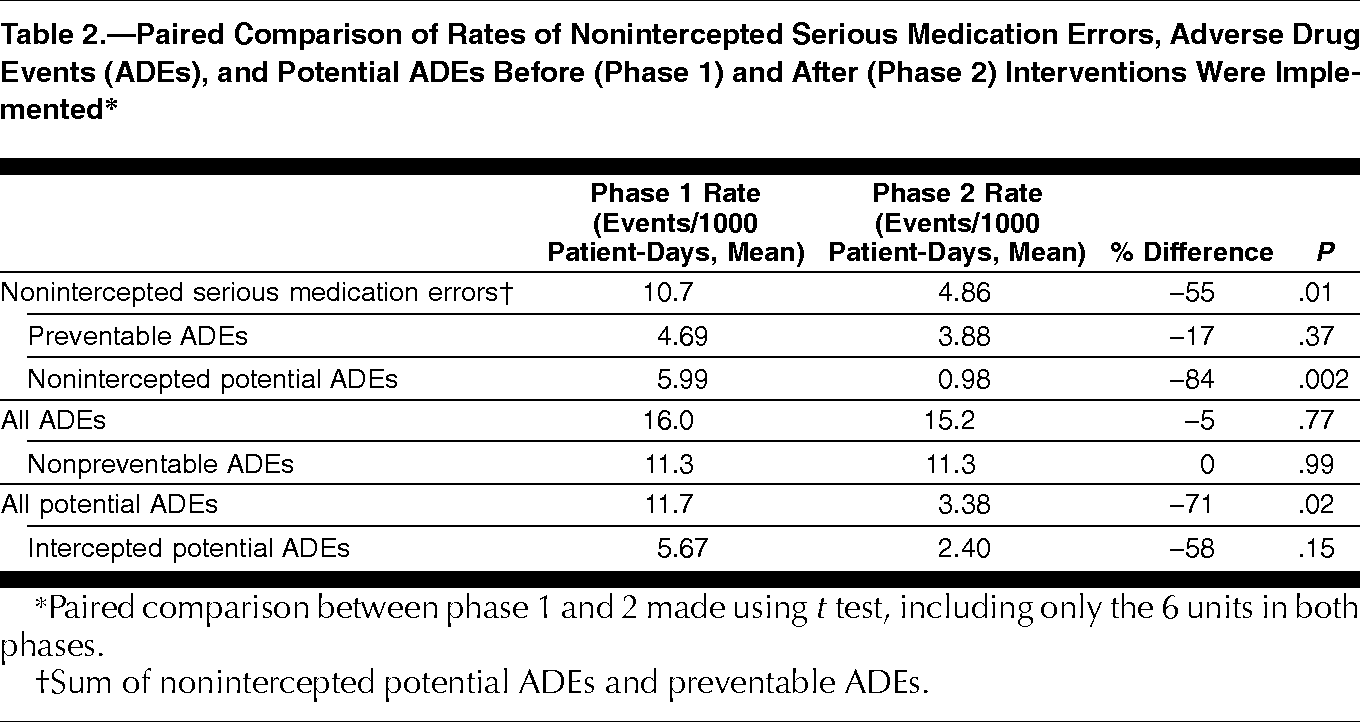
\includegraphics[width=0.8\textwidth]{images/jama2.png}
%	\end{center}
%	
%	\begin{itemize}
%		\item Does these differences seem reasonable?
%		\item Are there any other broad categories which they should have included?
%	\end{itemize}
%\end{frame}

%\begin{frame}{Reductions by Severity}
%	\begin{center}
%		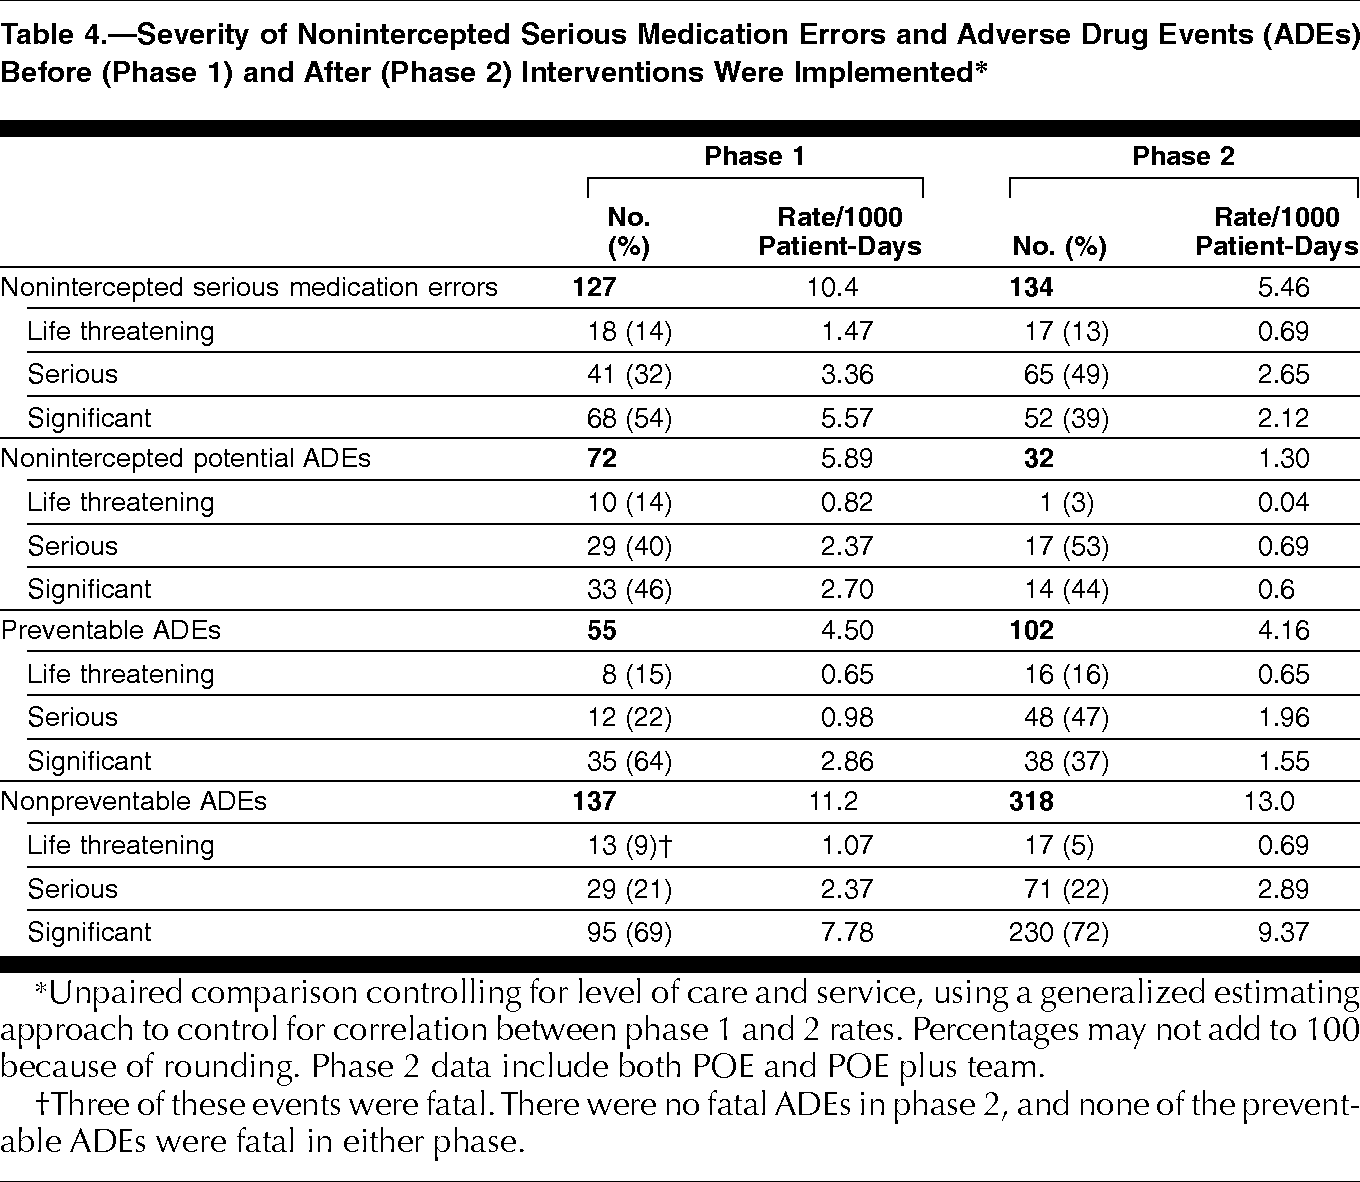
\includegraphics[width=0.8\textwidth]{images/jama4.png}
%	\end{center}	
%\end{frame}

%\begin{frame}{Reductions by Error Type}
%	\begin{center}
%		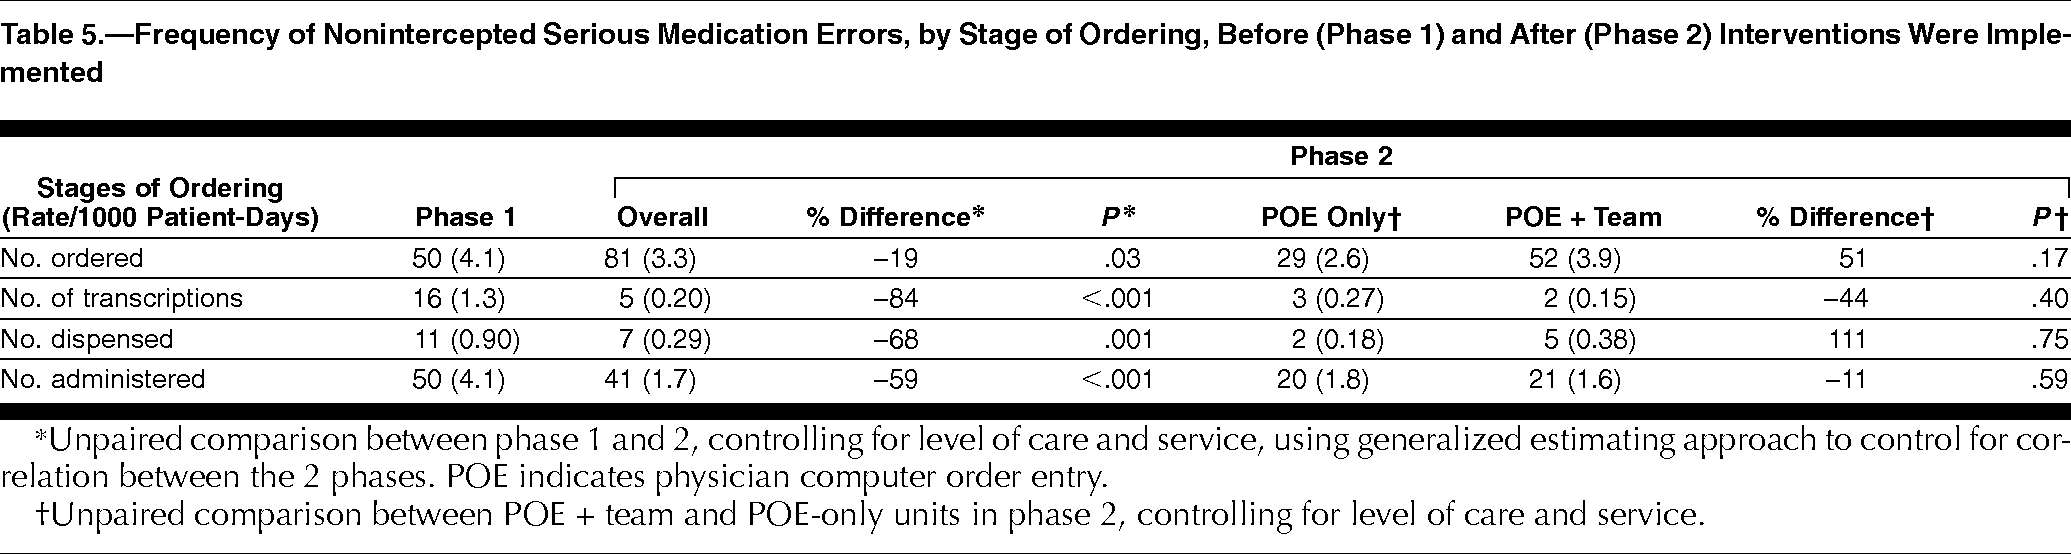
\includegraphics[width=0.8\textwidth]{images/jama5.png}
%	
%		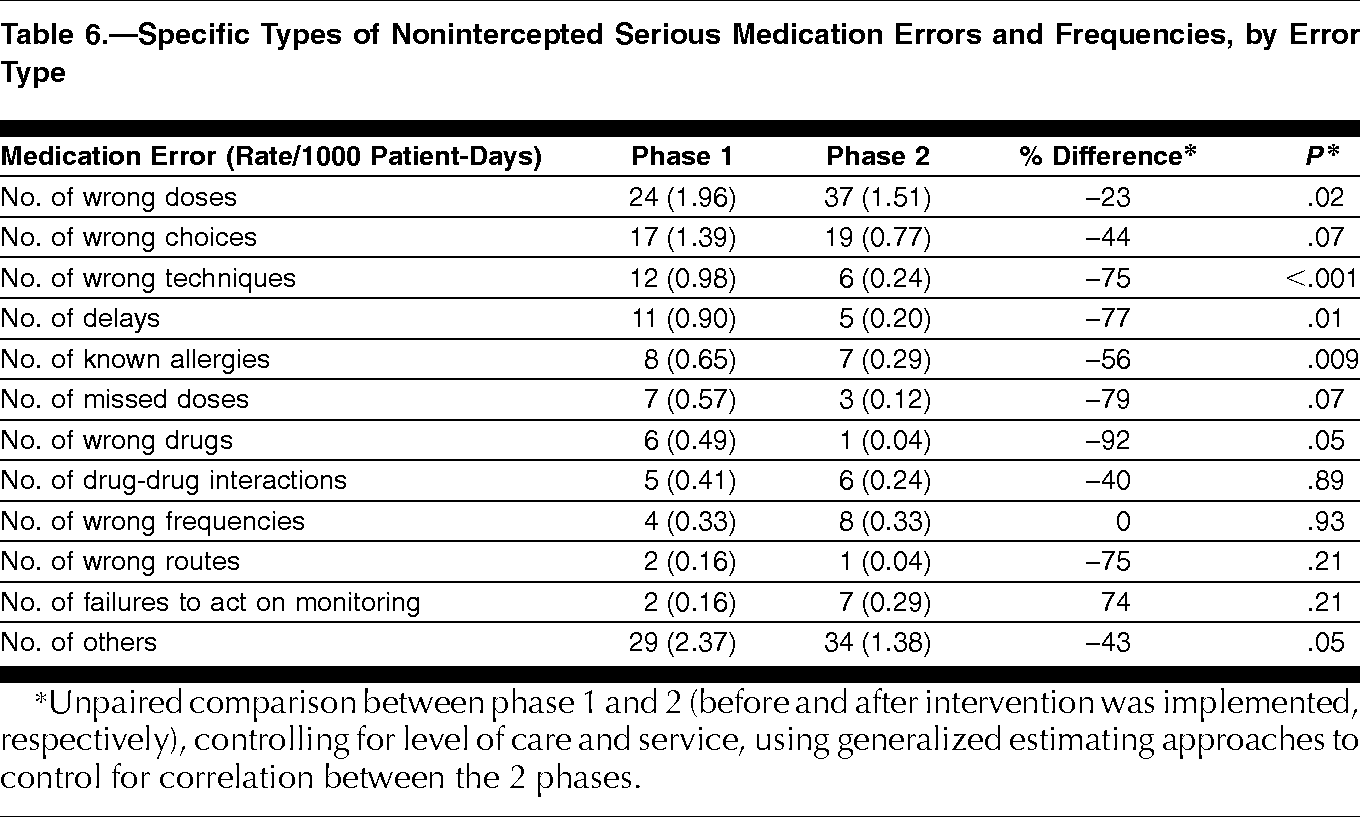
\includegraphics[width=0.8\textwidth]{images/jama6.png}
%	\end{center}
%\end{frame}

\begin{frame}{Reductions by Drug Type}
	\begin{table}
		\scriptsize
		\begin{tabular}{l c c c c}
			& Phase 1 & Phase 2 & \% Difference & $P$  \\ \hline \hline
			Analgesics & 2.05 & 1.14 & -44 & 0.01 \\
			Antibiotics & 1.72 & 0.86 & -50 & 0.04 \\
			Sedatives & 0.49 & 0.98 & +99 & 0.38 \\
			Antineoplastics & 0.49 & 0.24 & -50 & 0.34 \\ 
			Cardiovascular Drugs & 0.25 & 0.08 & -67 & 0.08 \\
			Anticoagulants & 0.98 & 0.24 & -75 & 0.01 \\
			Antipsychotics & 0.41 & 0.16 & -60 & 0.15 \\
			Diabetic Drugs & 0.49 & 0.24 & -50 & 0.49 \\
			Electrolytes & 0.90 & 0.20 & -77 & < 0.001 \\
			Others & 2.62 & 1.59 & -39 & 0.007 \\			
		\end{tabular}
		\caption*{Unpaired comparison of mean rates (events per 1000 patient days), controlling for level of care and service, using generalized estimating approaches to control for correlation between phases}
	\end{table}
\end{frame}


%\begin{frame}{Reductions by Drug Type}
%	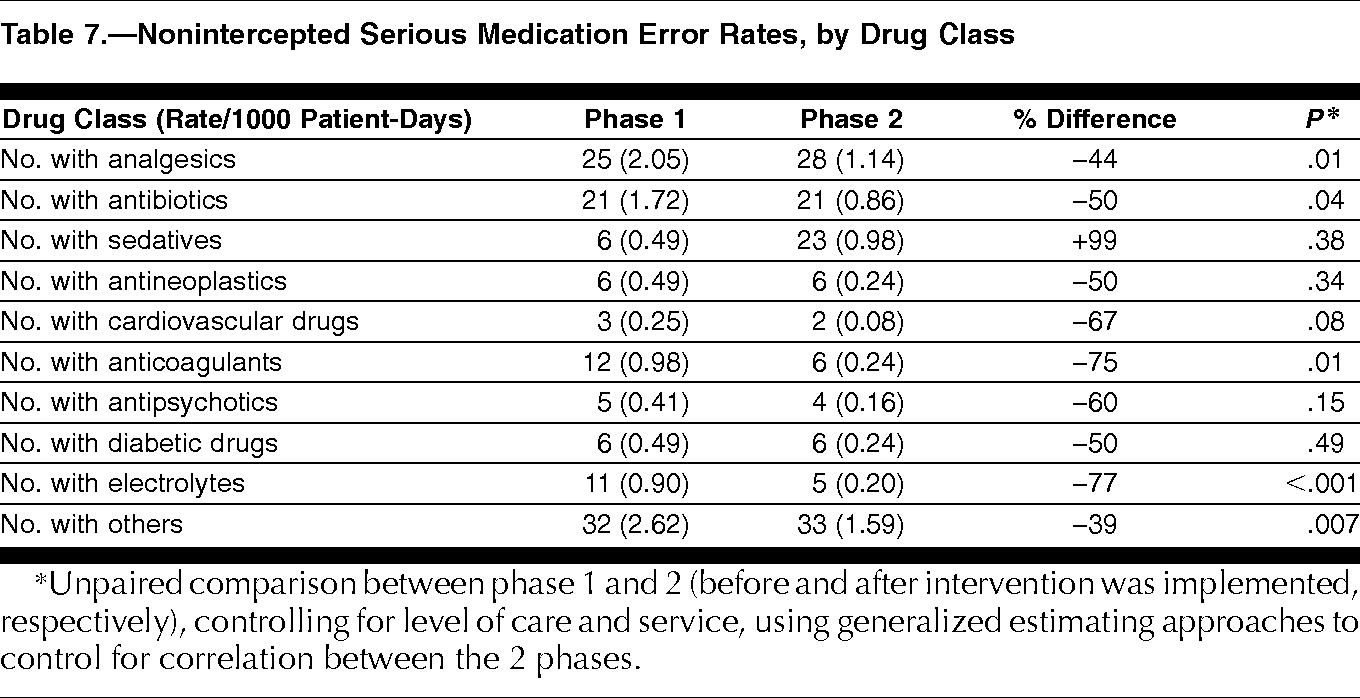
\includegraphics[width=1\textwidth]{images/jama7.png}
%\end{frame}

\begin{frame}{Economic Savings}
	\begin{itemize}
		\item Estimated annual costs of preventable ADEs of \$2.8 million. 
		\item If the observed 17\% decrease in the preventable ADE were the hospital-wide decrease, the annual savings would be \$0.48 million. 
		\begin{itemize}
			\item This does not include the costs of injuries borne by patients, of admissions due to drug errors, of malpractice suits, or of the extra work generated by the nonserious medication errors. 
		\end{itemize}
		\item The costs of developing and implementing POE have been estimated to be \$1.9 million, with maintenance costs of \$0.5 million per year
		\item The net savings have been estimated to be between \$5 to \$10 million per year.
	\end{itemize}
\end{frame}


\begin{frame}
	\begin{center}
 		{\Huge Thank You}
 		
 		\vspace{2cm}
 		This was a pilot lecture for a course to be given in the fall so any feedback is very much appreciated.
 		
 		\vspace{1.5cm}
 		
 		msnow1@montefiore.org
	\end{center}

\end{frame}

\end{document}